\section{Analysis}

\subsection{Logistic Regression Models}

\subsubsection{Methodology}

The fishing dataset, as prepared in the previous section, was used to model the probability of observing each of the six species.
A separate regression model was computed for each species, all taking on the following form:\linebreak

\tabto{2cm} ${Logit}(pi) = \beta_0 + \beta_{lat} x_{lat,i} + \beta_{lng} x_{lng,i} + \beta_{dpt} x_{dpt,i}$

\begin{itemize}
    \item Where $\beta_{0}$ is the model intercept
    \item and $x_{lat, i}$ is the latitude of the $i$-th observation in the dataset, measured in decimal degrees
    \item and $x_{lng, i}$ is the longitude of the $i$-th observation in the dataset, measured in decimal degrees
    \item and $x_{dpt, i}$ is the elevation / depth of the $i$-th observation in the dataset, measured in meters
    \item and $\beta_{lat}$, $\beta_{lng}$, $\beta_{dpt}$ are the model coefficients for latitude, longitude and depth, respectively
    \item and ${Logit}(pi)$ is the link function output for the $i$-th observation of the dataset.
\end{itemize}

The models were computed using the Python $statsmodels$ package.
A column of ones was added to the dataframe of predictor in order to represent the intercept.
The resulting model for each species was then used to calculate the estimated probability of detection for each point in the dataset.
This was achieved using the resulting model's $predict$ method.
Next, plots were generated for each species, displaying the relationship between the $Logit(p)$ function and the estimated probability of detection.
prior to plotting, the rows of the data were sorted by the estimated probability in ascending order.
In the same graphs, the observed presence-absence values were plotted in order to provide a sense of the distribution
of the estimated probabilities across the true values.
Boxplots displaying the same distribution of probably across the true presence-absence value were also generated.

Receiver operator curves (ROCs) were generated for each species-model.
The ROC helps to understand the trade-offs in selecting for different discrimination thresholds in terms of obtaining true positives vs.
false positives.
Obtaining more true positives means that you have to be willing to accept the probability of receiving false positives.
For each ROC, the area under the curve (AUC) is calculated.
As noted in our course module, a model with an AUC less than 0.5 performs worse than a random estimator.
The larger the AUC, the better the model performance.

Finally, the main output of this analysis is a distribution map for each species' occurrence in the southern Gulf of St. Lawrence.
For each coordinate in the data array, a corresponding estimate of probability of detection is calculated.
The heat map provides a way to visualize the estimated probabilities over the landscape.
In order to do this, I flattened the elevation data array into a pandas dataframe with the following columns: $const$, $latitude$, $longitude$, $elevation$.
Then, once again using the model's \textbf{predict} method, I calculated the estimated probability of occurrence for each row.
The resulting series of probability was then reshaped into the original ndarray shape of the elevation data array and inserted into a
new data array containing the same coordinates as the original.
These data arrays were then plotted using a heatmap theme color mapping.
Finally, the true occurrences were overlain the heat map to provide a visual sense of model performance.


\subsubsection{Results}

The estimates coefficients for each model for the intercept, $latitude$, $longitude$ and $depth$ are presented in Figure~\ref{fig:reg_coefs}.
The estimated coefficients for all predictors were observed to be statistically significant at the $\alpha=0.001$ level for each species
and thus retained in the final model.

The resulting $Logit(p)$ vs. estimated probability plots for each model is presented in Figure~\ref{fig:logitplots}.
Visual inspection of the plots gives us a sense about how effective the resulting models will be at effectively

The distribution of estimated probabilities across the observed presence-absence values are presented in Figure~\ref{fig:boxplots}.

The ROC plots for each species-model is presented in Figure~\ref{fig:rocs}.
The shapes and corresponding AUCs are indicative of the performance of each model.
All the computed AUCs are well-above 0.5, indicated that these models have at least some degree of usefulness.
The two most powerful models produced were for Redfish and Lobster which had AUCs of 0.90 and 0.95, respectively.
The least powerful model was for Snow Crab which had an AUC of 0.67.
A table of computed discrimination thresholds for each model are presented in Figure~\ref{fig:regression_discr_ths}.
Finally, the resulting distribution map for each species in the sGSL is presented in Figure~\ref{fig:heat_maps}.


\begin{figure}
    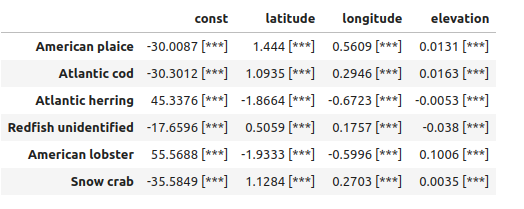
\includegraphics[width=\linewidth]{regression_coef_table}
    \caption{
        The estimated model coefficients for the intercept, latitude, longitude and elevation/depth for all six species.
        All coefficient in all models were observed to be significant at the $\alpha=0.001$ level, as indicated by the three asterisks
    }
    \label{fig:reg_coefs}
\end{figure}




\begin{figure}
    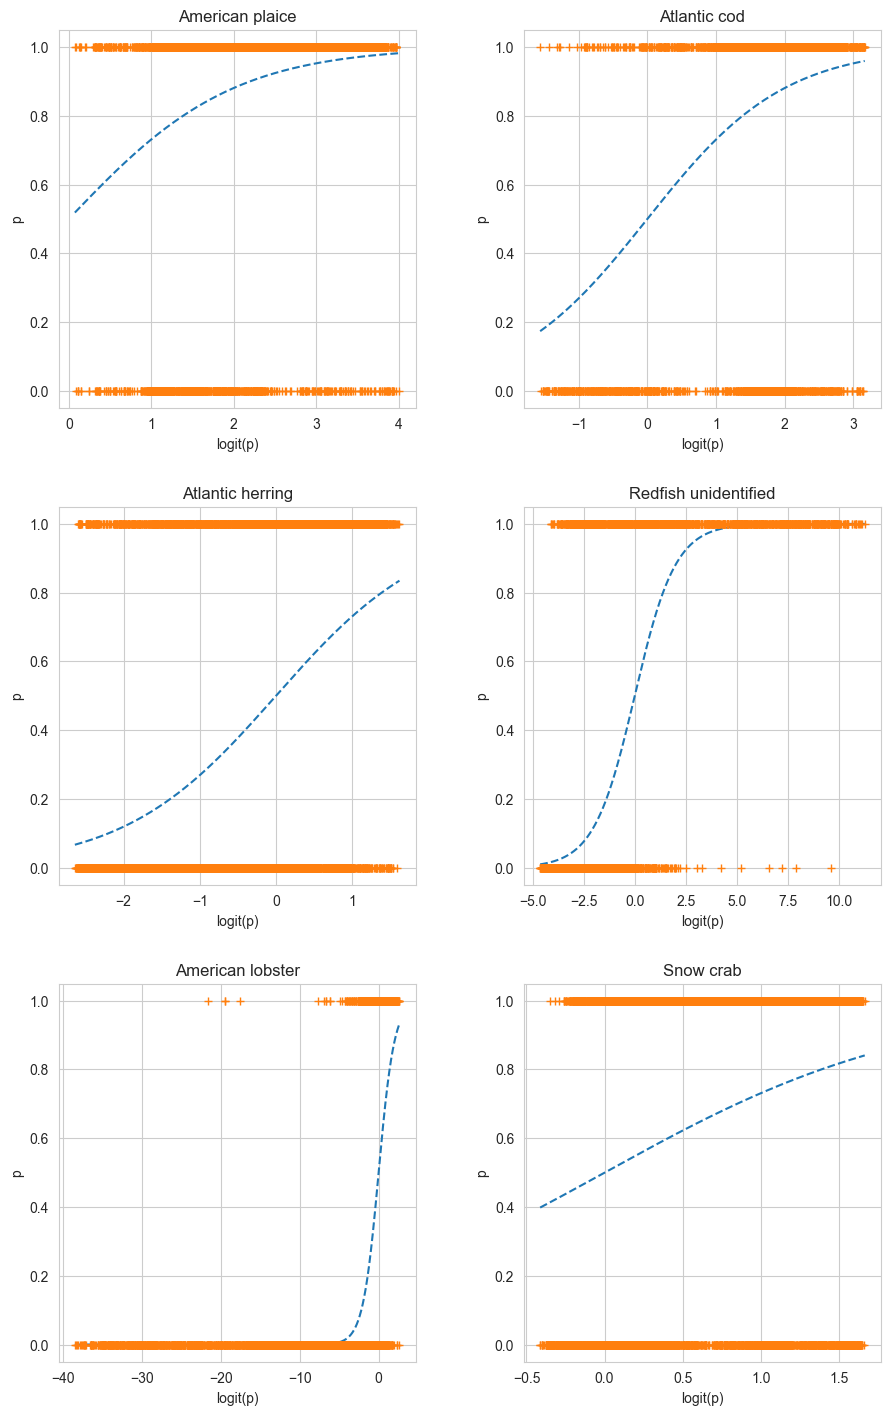
\includegraphics[height=18cm,keepaspectratio]{logitplots}
    \caption{
        Plots displaying $Logit(p)$ vs. estimated probabilities for each resulting model.
        Prior to plotting, the dataset was sorted in ascending order of estimated probability.
        The observed presence-absence values are superimposed on the plot in order to provide a sense of the
        distribution of true values accross estimated probabilities.
    }
    \label{fig:logitplots}
\end{figure}


\begin{figure}
    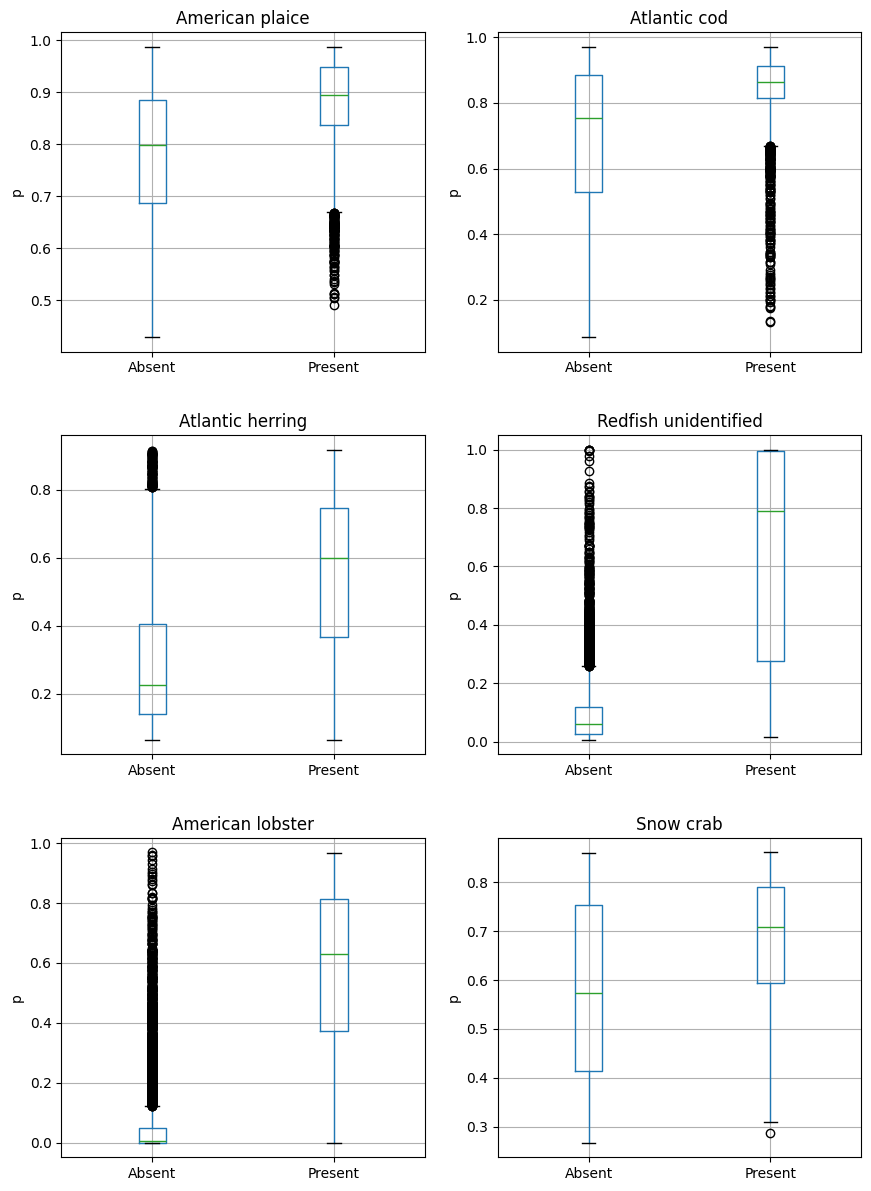
\includegraphics[height=18cm,keepaspectratio]{boxplots}
    \caption{
        A boxplot for each species model that shows the distribution of estimated probabilities for presences vs. absences.
    }
    \label{fig:boxplots}
\end{figure}



\begin{figure}
    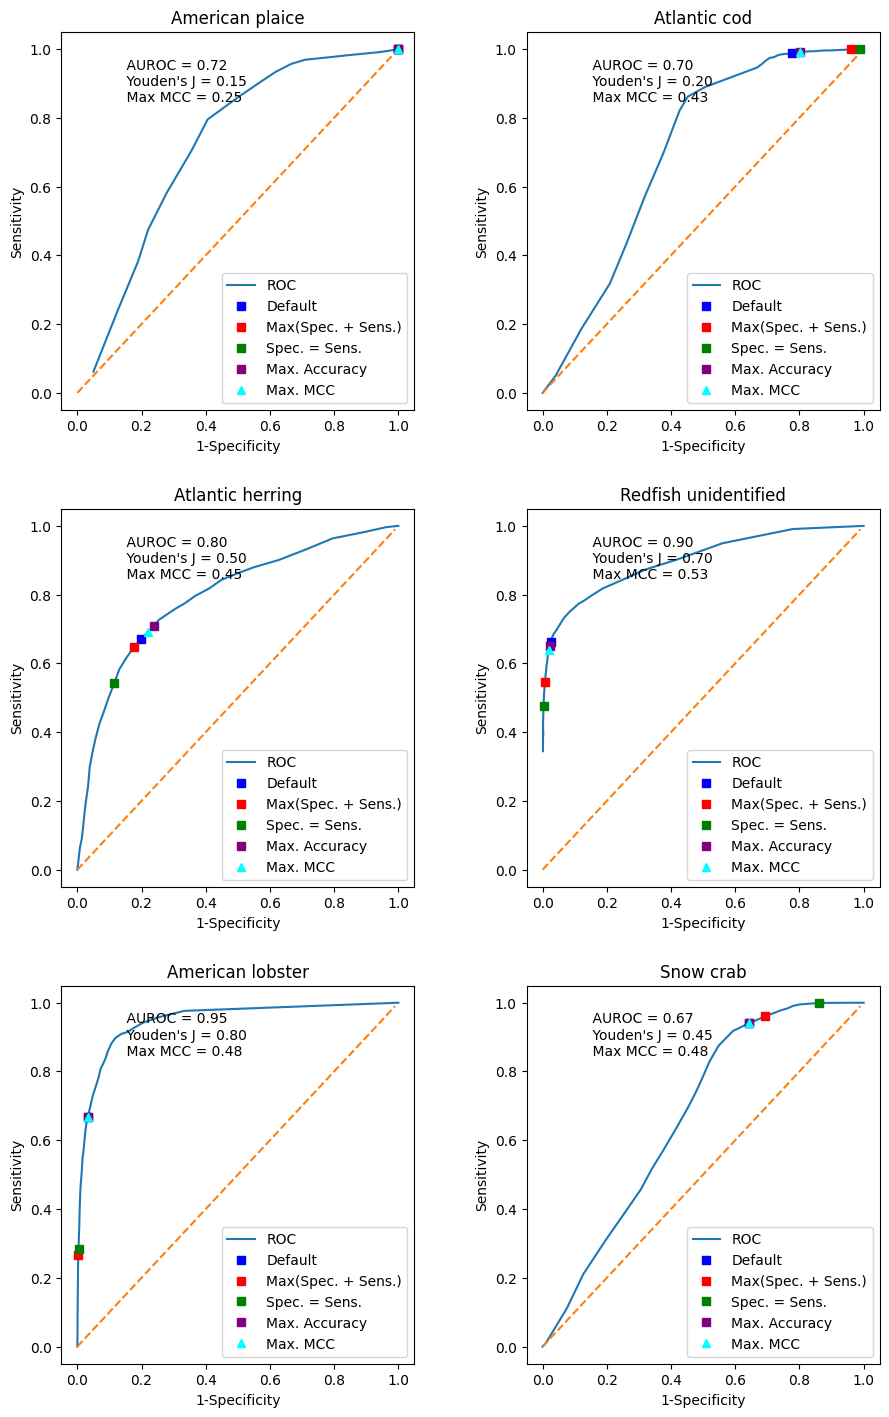
\includegraphics[height=18cm,keepaspectratio]{rocs}
    \caption{
        The receiver operator curves (ROC) for each species model.
        The area under the curve (AUC), Youden's J threshold and max MCC threshold are shown for each graph.
        These graphs display the trade-off between obtaining true positives and false positives when selecting different discrimination thresholds.
    }
    \label{fig:rocs}
\end{figure}



\begin{figure}
    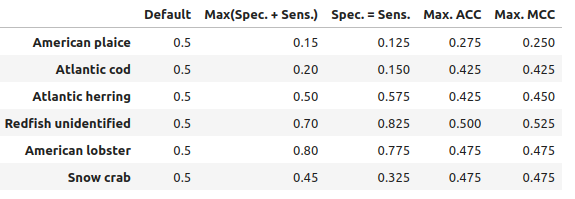
\includegraphics[width=\linewidth]{regression_discr_ths}
    \caption{
        A table key discrimination thresholds for each species model.
    }
    \label{fig:regression_discr_ths}
\end{figure}



\begin{figure}
    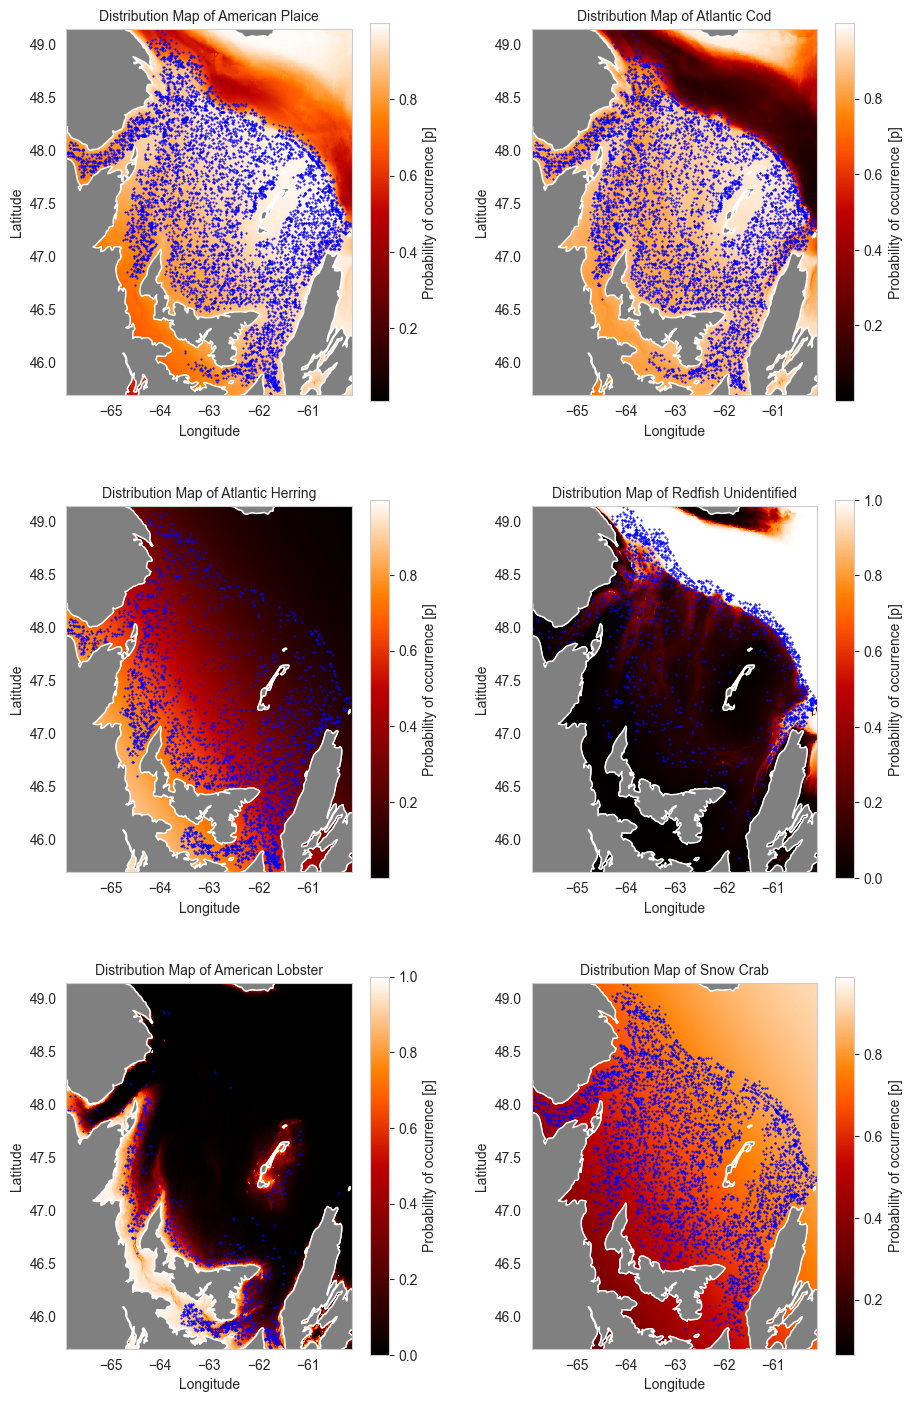
\includegraphics[height=18cm,keepaspectratio]{heat_maps}
    \caption{
        Distribution maps for all six species.
        Each map displays the inferred estimated probability for each point on the map and is depicted using a heatmap themed color mapping.
        The true occurrences for each species are overlain in order to provide a visual sense of model's performance.
    }
    \label{fig:heat_maps}
\end{figure}


